\documentclass[a4paper,ngerman,headsepline, titlepage=firstiscover]{scrartcl}
\KOMAoptions{fontsize=12pt}
\KOMAoptions{headings=standardclasses}
\KOMAoptions{DIV=13}
%\KOMAoption{captions}{centeredbeside}
\usepackage{scrlayer-scrpage}
\KOMAoptions{autooneside=false,automark}
\pagestyle{scrheadings}
\usepackage{scrdate,scrtime}

% LOCALISATION
\usepackage[utf8]{inputenc}
\usepackage[T1]{fontenc}
\usepackage[ngerman]{babel}
\usepackage[style=german,german=guillemets]{csquotes}
\pdfminorversion=7
\usepackage{calc}

% LAYOUT
\usepackage[activate=true,final,spacing=true,expansion=true]{microtype}

% VISUAL
\usepackage{amsmath,amssymb,amsfonts}
\usepackage{libertine}
\usepackage{inconsolata}
\usepackage{booktabs}
\usepackage{lastpage,multicol}
\usepackage{subcaption,setspace,enumerate}

% TOOLS
\usepackage[dvipsnames]{xcolor}
\usepackage{pgf,tikz}
\usepackage{siunitx}
\usepackage{listings}
\sisetup{locale=DE,per-mode=symbol,output-decimal-marker={,},detect-weight}

% PAGE LAYOUT
%\numberwithin{equation}{subsection}
\renewcommand*{\pagemark}{} % suppress center pagenum
\renewcommand{\thefootnote}{\roman{footnote}}
\setkomafont{pageheadfoot}{\rmfamily}
\clearpairofpagestyles
\lohead{Benutzerhandbuch \textit{htl-tk-chat}}
\rohead{Alexander Lessacher, Laurenz Preindl, Simon Graber}
\cohead{}
\rofoot{Seite \thepage\ von \pageref{LastPage}}

\newcommand*\diff{\mathop{}\!\mathrm{d}}

% BIBLIOGRAPHIE
%\usepackage[imakeidx]{xindex} % oldindex
\usepackage{makeidx}\makeindex
%\usepackage[backend=biber,style=authoryear,natbib=true,hyperref=true]{biblatex}
%\addbibresource{/home/ln/Dokumente/tex/literatur/main.bib}

\usepackage[hidelinks]{hyperref}
\usepackage{marvosym}
\hypersetup
{%
  pdfauthor={Graber, Preindl, Lessacher},%
  pdfcreator={pdfLaTeX}%
  colorlinks=true,linkcolor={black!70!blue},citecolor={blue!50!black},urlcolor={blue},%
  pdffitwindow={false},pdfstartview={FitH},%
  pdftitle={Dokumentation htl-tk-chat},pdfsubject={Software-Engineering}%
}

\hypersetup{%
    colorlinks,
    citecolor = {black!65!blue},
    filecolor = black,
    linkcolor = {black!50!blue},
    urlcolor = blue
}

\definecolor{backcolour}{rgb}{0.95,0.95,0.92}
\definecolor{codegray}{rgb}{0.5,0.5,0.5}
\definecolor{background}{HTML}{EEEEEE}
\definecolor{delim}{RGB}{20,105,176}
\colorlet{numb}{magenta!60!black}
\colorlet{punct}{red!60!black}
\lstdefinestyle{simple}{
    backgroundcolor=\color{backcolour},
    commentstyle=\color{green},
    keywordstyle=\color{red},
    numberstyle=\tiny\color{codegray},
    stringstyle=\color{purple},
    basicstyle=\ttfamily,
    breakatwhitespace=false,
    breaklines=true,
    captionpos=b,
    keepspaces=true,
    numbers=none,
    showspaces=false,
    showstringspaces=false,
    showtabs=false,
    tabsize=2,    
    literate=%
  {Ö}{{\"O}}1
  {Ä}{{\"A}}1
  {Ü}{{\"U}}1
  {ß}{{\ss}}1
  {ü}{{\"u}}1
  {ä}{{\"a}}1
  {ö}{{\"o}}1
}

\begin{document}

%\subject{}
\title{Handbuch \texttt{htl-tk-chat}}
\subtitle{Projekt: Fachspezifische Softwaretechnik}
\author{Simon Graber \and Laurenz Preindl \and Alexander Lessacher}

\maketitle
\tableofcontents
\newpage

\section{Einführung}
Der \texttt{htl-tk-chat} ist eine Chat-Applikation mit Qt-User-Interface. Sie können sich damit mit einem Client zu einem Server verbinden und mit den Teilnehmern dort Nachrichten austauschen. Standardmäßig geschieht dies verschlüsselt (SSL/TLS), ihre Nachrichten sind also auf dem Weg zu den anderen Teilnehmern \enquote{sicher}. Bilder der Applikation in dieser Anleitung wurden mit einem Breeze Dark Theme aufgenommen. Darstellung bei Ihnen kann sich unterscheiden.

\section{Abhängigkeiten}
Der Client hat folgende Abhängigkeiten:
\begin{itemize}
 \item Python >= 3.6
 \item PyQt5 >= 5.0
 \item python-msgpack
\end{itemize}

\noindent Der Server hat folgende Abhängigkeiten:
\begin{itemize}
 \item Python >= 3.6
 \item python-msgpack
\end{itemize}

\subsection{Installation}
\subsubsection{Python}
\paragraph{Windows} In Windows installieren Python Sie entweder über die \href{https://python.org}{Python} Webseite oder über winget mit folgendem Befehl:

\begin{lstlisting}[style=simple]
 winget install -e --id Python.Python
\end{lstlisting}

\paragraph{Debian:} In Debian basierenden Distributionen installieren Sie python über apt mit folgendem Befehl:

\begin{lstlisting}[style=simple, language=Bash]
 sudo apt install python3
\end{lstlisting}

\paragraph{ArchLinux:} In ArchLinux basierenden Distributionen installieren Sie python über pacman mit folgendem Befehl:

\begin{lstlisting}[style=simple, language=Bash]
 sudo pacman -Sy python
\end{lstlisting}

\subsubsection{PyQt5}
\paragraph{Windows:} In Windows installieren Sie PyQt5 mit Hilfe von pip nachdem Sie python installiert haben, mit folgendem Befehl:
\begin{lstlisting}[style=simple]
 pip install PyQt5
\end{lstlisting}

\paragraph{Debian:} In Debian basierenden Distributionen installieren Sie PyQt5 auch mit Hilfe von pip mit folgendem Befehl.
\begin{lstlisting}[style=simple]
 pip install PyQt5
\end{lstlisting}

\paragraph{ArchLinux:} In ArchLinux basierenden Distributionen können Sie PyQt5 über den Standard Weg mittels pacman installieren. Geben Sie dafür einfach folgenden Befehl ein:
\begin{lstlisting}[style=simple]
 sudo pacman -Sy python-pyqt5
\end{lstlisting}

\subsubsection{python-msgpack}
\paragraph{Windows:} In Windows installieren Sie python-msgpack mit Hilfe von pip nachdem Sie python installiert haben, mit folgendem Befehl:
\begin{lstlisting}[style=simple]
 pip install msgpack
\end{lstlisting}

\paragraph{Debian:} In Debian basierenden Distributionen installieren Sie python-msgpack auch mit Hilfe von pip mit folgendem Befehl.
\begin{lstlisting}[style=simple]
 pip install msgpack
\end{lstlisting}

\paragraph{ArchLinux:} In ArchLinux basierenden Distributionen können Sie python-msgpack über den Standard Weg mittels pacman installieren. Geben Sie dafür einfach folgenden Befehl ein:
\begin{lstlisting}[style=simple]
 sudo pacman -Sy python-msgpack
\end{lstlisting}
\newpage
\section{Client}
\subsection{Start}
Es wird davon ausgegangen, dass Sie die Applikation als Client nutzen und ein bestehender Server bekannt und erreichbar ist.\\
Zum Starten des Programms rufen sie unter \texttt{frontend/client.py} auf. Hierzu können sie die Datei direkt aufrufen (\texttt{./frontend/client.py}) oder dem Programm \texttt{python3} als Parameter übergeben. Hierzu verwenden sie den Befehl \texttt{python3 frontend/client.py}.

\begin{figure}[!h]\centering
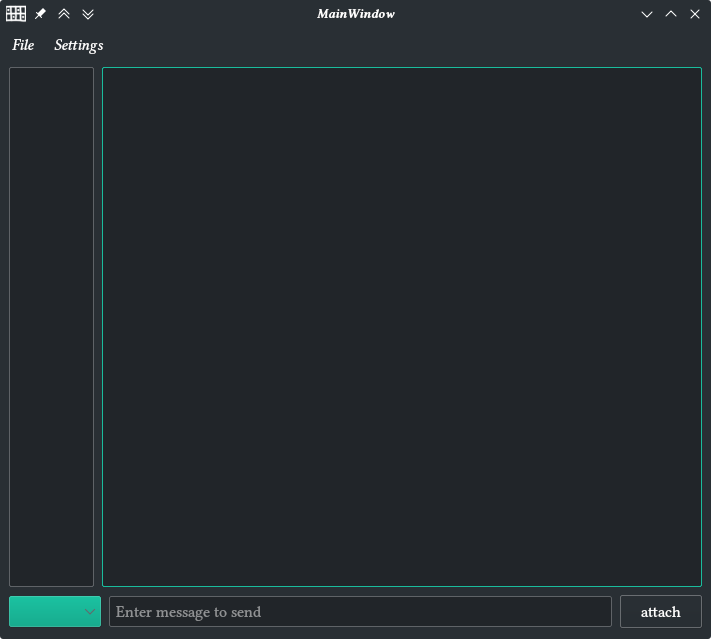
\includegraphics[width=\textwidth]{images/empty}
\caption{Hauptfenster nach dem Start}
\end{figure}

\newpage

\subsection{Konfiguration}
Wenn Sie noch keine Konfiguration haben öffnet sich beim ersten Start automatisch ein Einstellungsfenster in dem Sie eine Konfiguration einstellen können. Die Felder von Links nach Rechts sind: Serveradresse (Die IP Adresse oder Hostname des Servers), Port (Port des Servers Standard: 9999), Username (Der Name mit dem Sie im Chat angezeigt werden). Es gibt ebenfalls eine Checkbox für SSL. Wenn die Checkbox angeklickt ist versucht der Client eine verschlüsselte Verbindung zum Server aufzubauen. Mit dem Button \enquote{Save Profile} können Sie Ihre Konfiguration speichern. Mit \enquote{Delete Profile} können Sie Ihre Konfiguration auch wieder löschen. \enquote{Load Profile} lädt die gespeicherte Konfiguration in die entsprechenden Felder.
\begin{figure}[!h]\centering
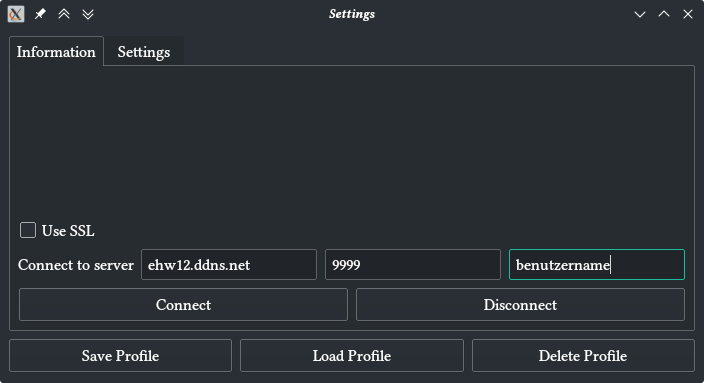
\includegraphics[width=\textwidth]{images/settings}
\caption{Einstellungsfenster\label{fig:settings}}
\end{figure}\clearpage
\newpage

\subsection{Nachrichten  Schreiben}
\noindent Nachdem Sie eingeloggt sind sehen Sie eine Nachricht vom Server. Links sehen Sie auch die aktuell verbunden Benutzer wie man in Abbildung \ref{fig:conversation} gut sehen kann. Um Nachrichten zu verfassen, tippen Sie den Text in die Eingabezeile am unteren Rand des Fensters ein und drücken die Enter-Taste. Um private Nachrichten zu versenden wählen Sie den Benutzer, an den Sie die Nachricht senden wollen. unten Links in der Combo Box aus.

\begin{figure}[!h]\centering
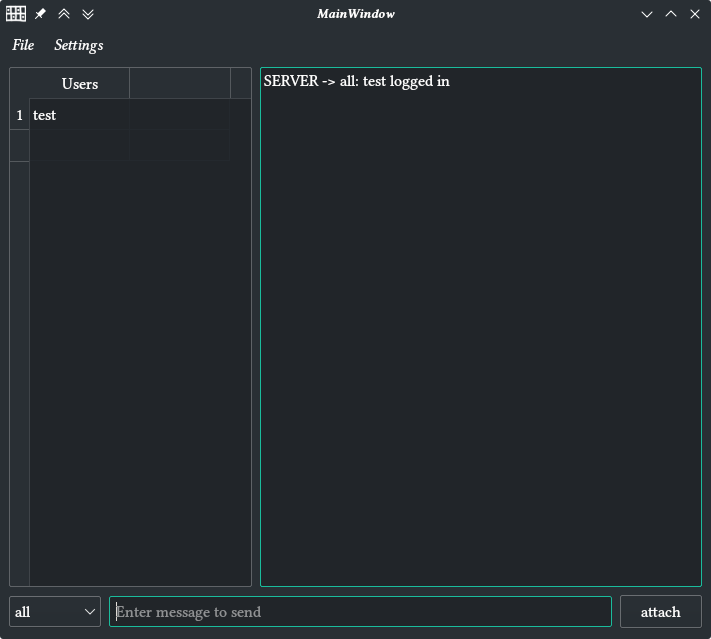
\includegraphics[width=\textwidth]{images/alone}
\caption{Login Nachricht \label{fig:alone}}
\end{figure}
\newpage

\begin{figure}[!h]\centering
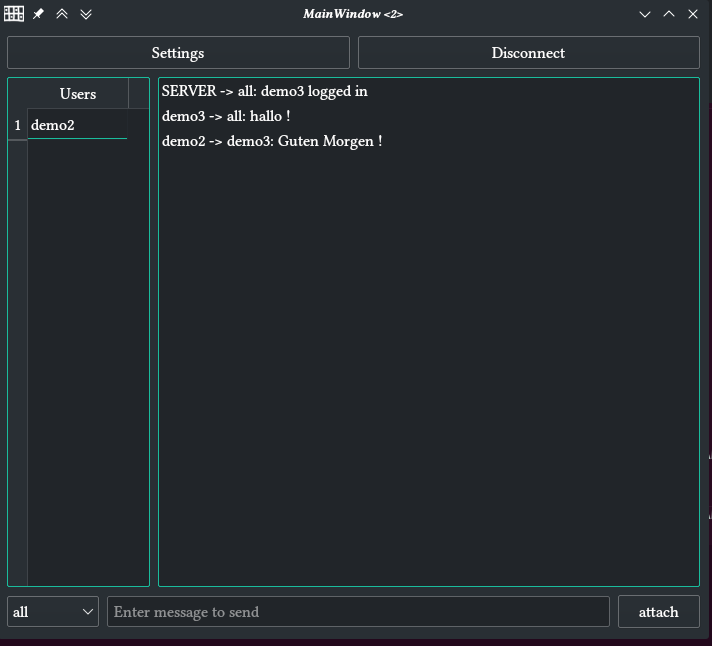
\includegraphics[width=\textwidth]{images/conversation}
\caption{Konversation\label{fig:conversation}}
\end{figure}
\newpage

\subsection{Bilder}

Der \texttt{htl-tk-chat} unterstützt Bilder im Chat. Die Bilder werden als Thumbnail mit einer maximal Größen von 300 mal 300 Pixel angezeigt. Um ein Bild zu versenden drücken sie unten Rechts auf den \enquote{attach} Button. Danach öffnet sich ein File Dialog mit einem Filter für Bild Dateien. Wählen Sie die gewünschte Bild Datei aus um Sie zu versenden.
\begin{figure}[!h]\centering
\includegraphics[width=\textwidth]{images/attach-image}
\caption{Bild in Chat\label{fig:attach-image}}
\end{figure}
\newpage

\subsection{Dateien}

Der \texttt{htl-tk-chat} unterstützt auch das versenden von Dateien. Um eine Datei zu versenden verwenden Sie wie bei Bildern den \enquote{attach} Button unten Rechts. Danach öffnet sich ein File Dialog. Im File Dialog wählen Sie den Filter \enquote{All Files} aus um alle Dateien zu sehen. Danach wählen Sie eine Datei aus die kein Bild ist um sie zu versenden. Dateien werden im Chat wie eine normale Text Nachricht angezeigt, mit dem Unterschied, in der Nachricht steht \enquote{file: [Dateiname]}. Um die Datei herunterzuladen drücken Sie mit der Maus auf die Nachricht. Danach öffnet sich ein File Dialog zum speichern der Datei.
\begin{figure}[!h]\centering
\includegraphics[width=\textwidth]{images/file}
\caption{Bild in Chat\label{fig:attach-file}}
\end{figure}
\newpage
\section{Server}
\subsection{Start}
Zum Starten des Programms rufen sie unter \texttt{server/chat\textunderscore server.py} auf. Hierzu können sie die Datei direkt aufrufen (\texttt{./server/chat\textunderscore server.py}) oder dem Programm \texttt{python3} als Parameter übergeben. Hierzu verwenden sie den Befehl \texttt{python3 server/chat\textunderscore server.py}.

\subsubsection{Autostart}
Wenn Sie einen Chat Server betreiben wollen empfiehlt es sich diesen über ein Autostart System im Hintergrund zu starten. Wir empfehlen dazu die Verwendung von Systemd. Eine solche Systemd Service File kann folgendermaßen aussehen:
\begin{lstlisting}[style=simple]
[Unit]
Description=htl-tk-chat Server
After=network.target

[Service]
Type=simple
User=root
Group=htl-tk-chat
WorkingDirectory=/path/to/server/directory
ExecStart=/usr/bin/python3 /path/to/chat_server.py
Restart=on-failure

[Install]
WantedBy=multi-user.target
\end{lstlisting}

\subsection{Konfiguration}
Wenn Sie den Server starten benötigen Sie eine Konfigurationsdatei namens \enquote{server.conf} im selben Verzeichnis wie die \enquote{chat\textunderscore server.py} Datei. Wenn diese Datei nicht vorhanden ist erstellt der Server diese mit einer Standardkonfiguration. Diese Konfiguration sieht folgendermaßen aus:
\begin{lstlisting}[style=simple]
[SERVER]
listen_address = 0.0.0.0
listen_port = 9999

[SSL]
enable_ssl = False
keyfile = key.pem
certfile = cert.pem
\end{lstlisting}
Wenn Sie SSL Verschlüsselung für die Übertragung aktivieren wollen müssen Sie die \enquote{enable\textunderscore ssl} Konfiguration auf \texttt{True} bzw. 1 stellen. Außerdem müssen Sie den Schlüssel und das Zertifikat für die SSL Verschlüsselung angeben.
\subsection{Logging}
Der Server loggt die aktuelle Programmausführung mit. Die Logging Nachrichten sehen Sie im Terminal nachdem Sie den Chat Server gestartet haben und in der Datei \enquote{chatserver.log} im selben Verzeichnis wie \enquote{chat\textunderscore server.py}. Wenn Sie die Ausgabe der Log Nachrichten bearbeiten wollen können sie das in der Datei \enquote{logger.conf} im Verzeichnis des Chat Servers. Die Standardkonfiguration sieht folgendermaßen aus:
\begin{lstlisting}[style=simple]
[loggers]
keys=root

[handlers]
keys=term,file

[formatters]
keys=iso

[logger_root]
level=NOTSET
handlers=term,file

[handler_term]
class=StreamHandler
level=NOTSET
formatter=iso
args=(sys.stdout,)

[handler_file]
class=FileHandler
level=NOTSET
formatter=iso
args=("./chatserver.log", "w")

[formatter_iso]
class=logging.Formatter
format=%(asctime)s %(levelname)s %(message)s
datefmt=%Y-%m-%dT%H:%M:%S%z 
\end{lstlisting}
Für mehr Information zur Konfiguration der Log Nachricht sehen Sie \href{https://docs.python.org/3/library/logging.config.html#configuration-file-format}{hier}.

\end{document}
